%%% final.tex
%%%
%%% This LaTeX source document can be used as the basis for your technical
%%% paper or abstract. Intentionally stripped of annotation, the parameters
%%% and commands should be adjusted for your particular paper - title, 
%%% author, article DOI, etc.
%%% The accompanying ``template.annotated.tex'' provides copious annotation
%%% for the commands and parameters found in the source document. (The code
%%% is identical in ``template.tex'' and ``template.annotated.tex.'')

\documentclass[conference]{acmsiggraph}

\usepackage{amsmath}
\usepackage{amssymb}
\TOGonlineid{45678}
\TOGvolume{0}
\TOGnumber{0}
\TOGarticleDOI{1111111.2222222}
\TOGprojectURL{}
\TOGvideoURL{}
\TOGdataURL{}
\TOGcodeURL{}

\title{Rendering Metaballs with PBRT}

\author{Vinícius Vendramini\thanks{e-mail:todo@email.com}\\IME-USP \and Wilson K. Mizutani\thanks{e-mail:kazuo@ime.usp.br}\\IME-USP}
\pdfauthor{Vinícius Vendramini, Wilson K. Mizutani}

\keywords{isosurface, metaball, mesh generation, ray tracing}

\begin{document}

%% \teaser{
%%   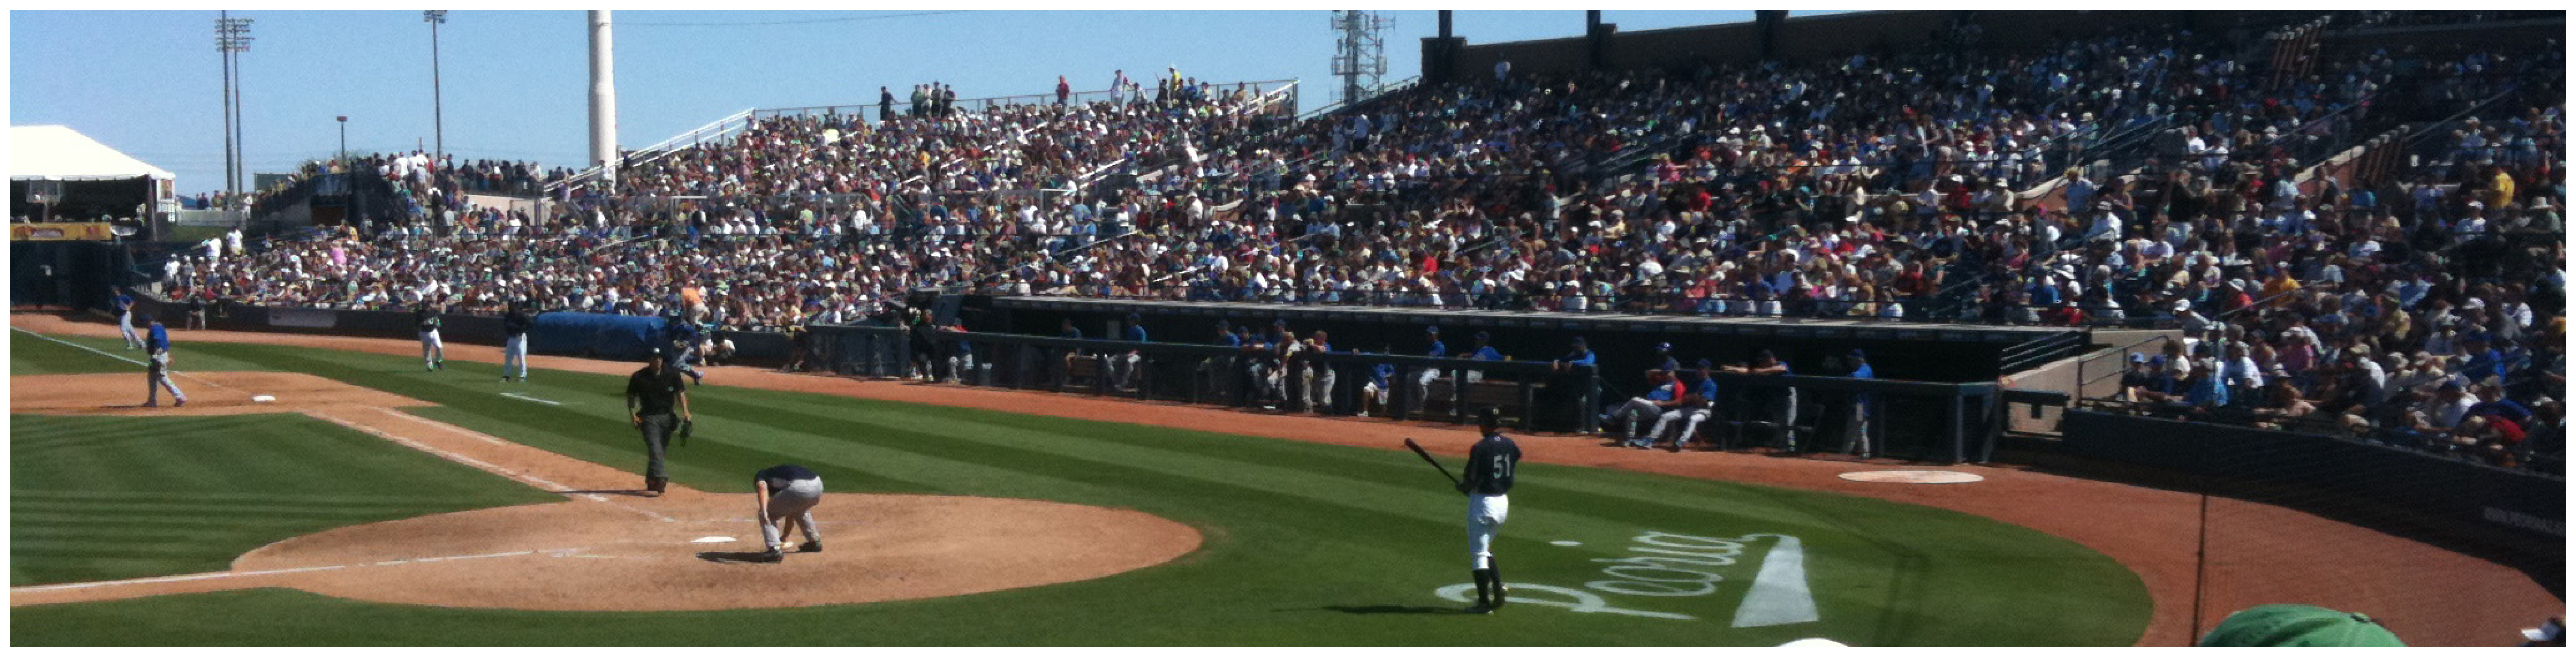
\includegraphics[height=1.5in]{images/sampleteaser}
%%   \caption{Spring Training 2009, Peoria, AZ.}
%% }

\maketitle

\begin{abstract}

Three dimensional geometry is often made through meshes, which requires
either modeling skills or data extraction from real bodies. This is specially
difficult for more organic or fluid structures, like creatures, liquids or
gases. Blinn \shortcite{Blinn:1982:GAS:965145.801290} proposes a way of defining
geometry through a particular type of isosurface that provides a simple
way of representing such geometries. These surfaces are known as
\textit{metaballs}. In this work we strive for a thourough renderization of
these geometries using the highly awarded PBRT
\shortcite{Pharr:2010:PBR:1854996} render system. There are two methods covered:
one based on Blinn's original intersection algorithm, and another using the
marching cubes algorithm \cite{Lorensen:1987:MCH:37402.37422} to generate a mesh
that approximates the surface. A few constraints on PBRT's architecture prevents
us from properly shading the metaballs materials, but nevertheless correctly
detects ray intersections. The \textit{marching cubes}, on the other hand, work
perfectly well, even without implementing all of its cases. It comes with a
rather high memory space cost though.

\end{abstract}

%\begin{CRcatlist}
%  \CRcat{I.3.3}{Computer Graphics}{Rendering Metaballs with PBRT}{Implicit surfaces}
%  \CRcat{I.3.7}{Computer Graphics}{Rendering Metaballs with PBRT}{Ray-tracing};
%\end{CRcatlist}

\keywordlist

%% Use this only if you're preparing a technical paper to be published in the 
%% ACM 'Transactions on Graphics' journal.

\TOGlinkslist

%% Required for all content. 

\copyrightspace

\section{Introduction}

There are many physical structures that can be described as being a composition
of bumps or blobs. A cloud, for instance, could be constructed as many smaller,
simpler clouds put together, merging in the regions between them. That is very
similar to what happens with electron densities when molecules form from
individual atoms: the resulting combined electrospheres combine where the atoms
join each other. Other examples could be liquids in general (the bumps would be
individual drops) or even flesh-based creature bodies (the blobs would ``grow''
from the bones). One way of defining this representation is through the use of
\textit{metaballs}, as seen in \cite{Blinn:1982:GAS:965145.801290} (the term
\textit{metaball} was not actually used in the original text).

\subsection{Metaballs}

Blinn \shortcite{Blinn:1982:GAS:965145.801290} defines a particular type of
isosurface that is a composition of simpler isosurfaces. An isosurface is the
set of points in $\mathbb{R}^n$ that solves the implicit equation
$F(x) = 0$ for a given function $F:\mathbb{R}^n \rightarrow \mathbb{R}$. For
example, the function $F(x) = \|x\|^{-1} - 1$ gives an isosurface
consisting of the unit hypersphere in $\mathbb{R}^n$. The surface Blinn presents
defines this $F$ in $\mathbb{R}^3$ as follows:

\begin{equation}
  F(x) = D(x) - T
\end{equation}

Where $T$ is a \textit{threshold} value (usually $1$) and
$D:\mathbb{R}^3 \rightarrow \mathbb{R}$ is the sum of $n$ exponentials, each
corresponding to an individual bump of the metaball:

\begin{equation}
  D(x) = \sum_{i=1}^{n} b_i e^{-a_i \|x-P_i\|}
\end{equation}

Where $P\in\mathbb{R}^3$ and $b_i,a_i\in\mathbb{R}$ for $i=1,...,n$. The
exponentials also represent spheres, with $P_i$ being their respective centers
and $a_i$ and $b_i$ factors that together determine the radius and how much each
bump clings to other bumps. Since these two coefficients are not very intuitive,
Blinn proposes a few change of variables, as well as using the squared distance
$\|x-P_i\|^2$ for code optimization. The resulting formula is:

\begin{equation}
  D(x) = \sum_{i=1}^{n} T e^{\frac{B_i}{R_i^2}\|x-P_i\|^2 - B_i}
\end{equation}

In this version, $R_i$ is the bump's radius, and $B_i$ is its blobbiness
factor, which must be negative. The closer to zero the blobbiness factor is,
the more merged and homogeneous neighbouring bumps become. Also, it is assumed
that $T=1$ in this form.

With the metaball representation, it is possible to build very complex fluid
geometries by simply placing various bumps (with possibly varying radiuses and
blobbiness) and using an aproppriate material, as seen in Figure
\ref{img:metaball-liquid}\footnotemark{}.

Another very important property of isosurfaces in general, is that if
$F(x)$ is differentiable, then a nonzero gradient $\nabla F$ at a point $x$ is
the surface normal at that point, towards the growing size. In the case of
Blinn's metaballs, the gradient gives an inwards normal, so for shading
purposes, $-\nabla F(x)$ is used.

\begin{figure}[ht]
  \centering
  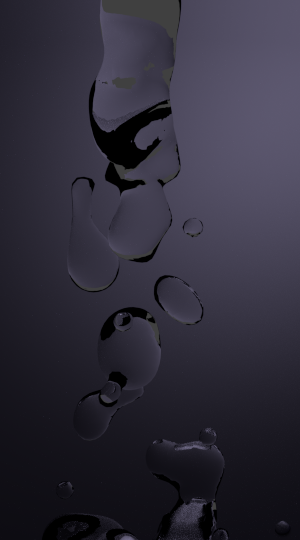
\includegraphics[width=1.5in]{images/fluid.png}
  \caption{Renderization of a liquid with metaballs.}
  \label{img:metaball-liquid}
\end{figure}

\footnotetext{
  This rendered image was made using the Blender Cycles Engine software with
  particle fluid simulation \cite{Blender}
}

\subsection{PBRT}

The \textit{Physically Based Ray-Tracer} is a tool developed together with a
text book \cite{Pharr:2010:PBR:1854996} for teaching global illumination methods
to graduate and post-graduate students. It is written in plain \texttt{C++},
using its own scene description file format for input and generating EXR images
\cite{EXR} as output. It provides a series of interfaces for extending the
system's features, so that students are able to develop new algorithms as CG
course projects.

As its name states, the PBRT system is centered on ray tracing algorithms that
try to render three-dimensional scenes while being as physically real as
acceptable by modern standards. Simply speaking, many rays are shot from a
virtual camera, bouncing off or going through the scene objects like real light
does upon reaching different kinds of materials. This achieves global
illumination better than classic CG architectures, such as OpenGL's pipeline, 
but is otherwise not as fast.

We are particularly interested in PBRT's \texttt{Shape} interface, because
through it we can provide an implementation for metaball rendering in PBRT.
There are mainly two types of shapes in it: intersectable and non-intersectable.
The first ones are able to determine whether a ray (from the ray tracing
algorithm) intersects with it, and the properties of the point of intersection,
i.e. its differential geometry information. The second type, not being able to
do the same, must be instead capable of refining itself into simpler shapes,
which can either be intersectable or not. This refination process goes on
recursevely until only intersectable shapes remain.

\subsection{Rendering methods}

Blinn's original work \shortcite{Blinn:1982:GAS:965145.801290} provides a way
for directly calculating a ray's intersection with a metaball. As we show
later, though, it does not work well with PBRT's architecture. We can only
achieve a partial result, mainly due to it not being possible to formulate a
global and generic parametrization for metaball surfaces.

An alternative we found was to use the marching cubes algorithm
\cite{Lorensen:1987:MCH:37402.37422}, also explained in further sections. With
it, we can derive triangle meshes from implicit functions using a
divide-and-conquer approach. The mesh approximates the original surface, its
error depending on the size of the \textit{cubes} used in the algorithm. In a
way, this is not actually rendering a metaball, but rather a procedure to
easily transform it into a very acceptable mesh. After that, PBRT can use its
own default shape \texttt{TriangleMesh} to properly render the resulting
geometry.

\section{Marching cubes algorithm}

\begin{figure}[ht]
  \centering
  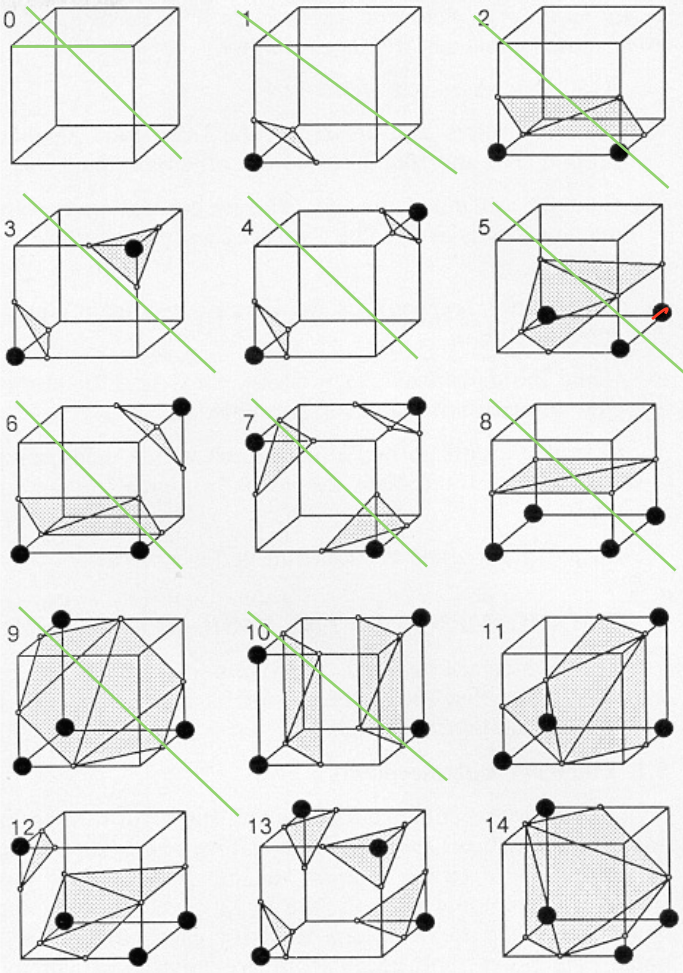
\includegraphics[width=3in]{images/base-cases}
  \caption{Representations of the fifteen cases, which can be rotated to form almost all posible triangulations of a marching cube.}
\end{figure}

The marching cubes algorithm \cite{Lorensen:1987:MCH:37402.37422} was introduced as an efficient way to render isosurfaces. Its divide-and-conquer approach sections the space that contains the surface into several much smaller cubes, which are then considered individually. As shown earlier, the nature of isosurfaces makes it easy to determine whether a point $x$ is on one side of the surface or the other by simply analysing whether the value of $D(x)$ is smaller or greater than the threshold $T$. Using that fact, the algorithm considers each cube and determines on which side of the isosurface lies each of the cube's 8 vertices.

This information is then used to determine which of several possible triangulations would best suit that particular cube. Since each of the 8 vertices has two possible states (one side or the other), there are $2^8 = 256$ possible triangulations, which are stored in a preprocessed table for easy access. Because many triangulations are simply rotated versions of other possibilities, they can be separated into \textit{families} or \textit{cases}, which gives a better understanding of their workings. These cases are divided into fifteen base cases and six complementary cases \cite{Lingrand}, which we show later. The way the cases are chosen guarantees that there will be no topological artifacts such as accidental holes in the resulting mesh.

\begin{figure}[ht]
  \centering
  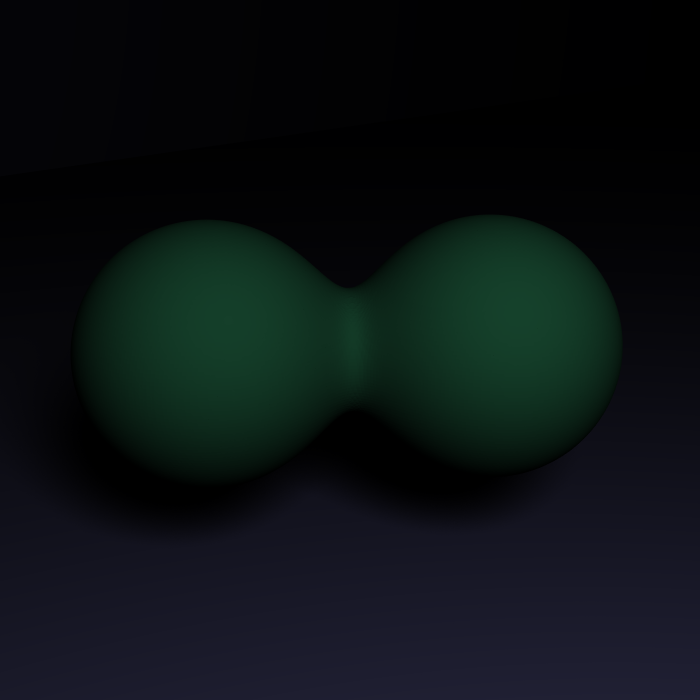
\includegraphics[height=1.5in]{images/metaball-non-interpolated}
  \caption{A pair of metaballs rendered without interpolation, putting the vertices of the triangles at exactly the middle of the cube's edges.}
  \label{img:non-lerp}
\end{figure}

Each triangulation is done by having at most one vertex of a triangle in any given edge of the cube. Using that, we can interpolate the values of $D(x)$ in that edge's vertices to determine whether the triangle should be closer to one vertex or the other. This allows for the triangles to have almost any inclination so that the resulting mesh is considerably smoother (compare Figure \ref{img:non-lerp} and Figure \ref{img:marching-cubes}). Since this cube's vertices will have the same value of $D(x)$ as the vertices of its neighbors, no holes are created in the mesh by the interpolation.

\subsection{Ambiguous cases}

\begin{figure}[ht]
  \centering
  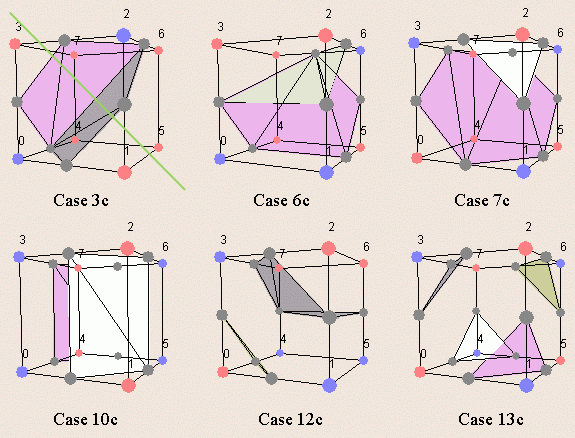
\includegraphics[width=3in]{images/ambiguous-cases}
  \caption{Representations of each of the complementary triangulations used to avoid problems in ambiguous cases.}
  \label{img:amb-cases}
\end{figure}

Each of the fifteen base cases has an associated \textit{complementary} case, which may be obtained by reversing the vertices' sides - if a vertex is on the inside of a base case it would be on the outside in its complementary, and vice versa. In most cases it is possible to use the same triangulation for the base case and its complementary. However, there are six cases out of the fifteen which require special attention, since using the same triangulation for the complementary case would cause holes to appear in the surface. These six cases are called \textit{ambiguous} and create the need for six additional triangulation possibilities (Figure \ref{img:amb-cases}). See Figure \ref{img:bad-comp} for an example.

\begin{figure}[ht]
  \centering
  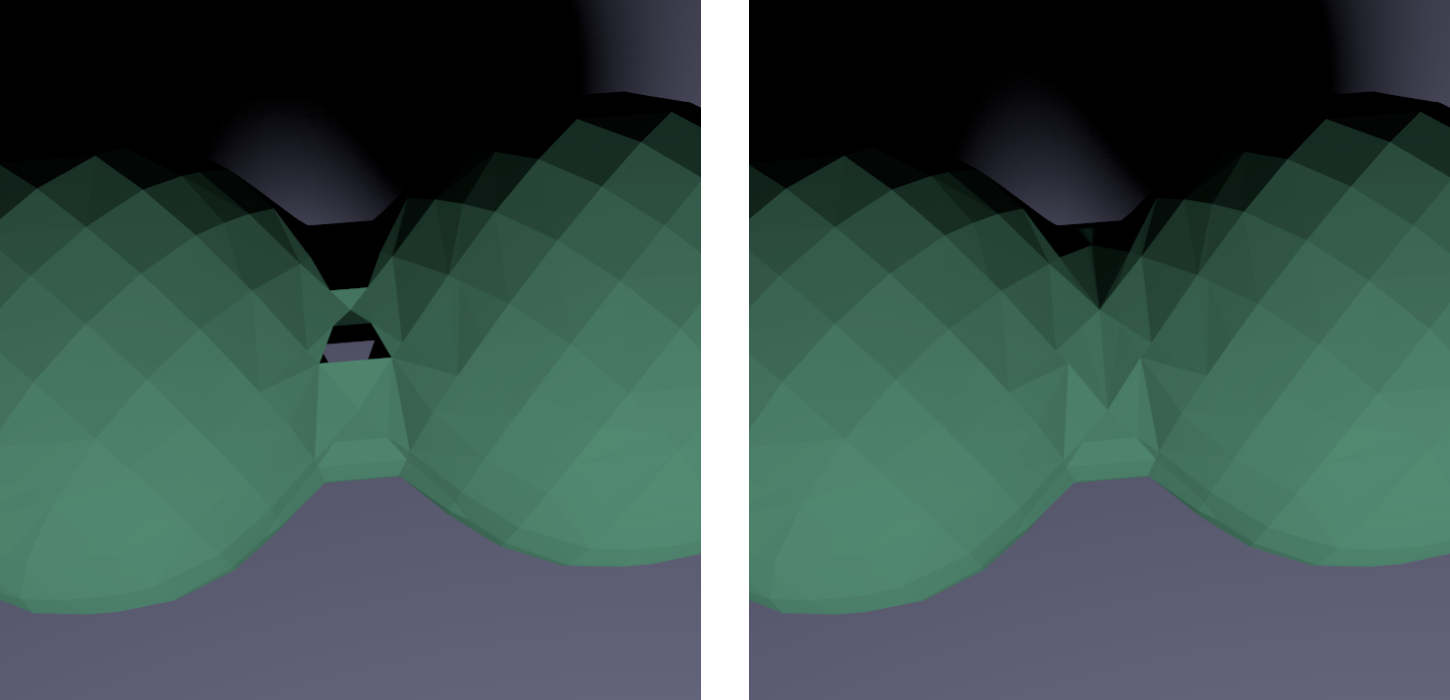
\includegraphics[height=1.5in]{images/metaball-bad1-comparison}
  \caption{On the left, a pair of metaballs rendered without considering the ambiguous cases, which results in an inappropriate triangulation and holes on the mesh; on the right, the same metaballs rendered with the additional triangulations used to cover the ambiguous cases. Both were rendered in ways that remove realism but clarify the problem.}
  \label{img:bad-comp}
\end{figure}

\section{Analytic intersection}

\section{Implmentation}

\subsection{PBRT limitations}

\section{Implementation}

In our project, we implemented both metaball rendering using both Blinn's
intersection algorithm (which is intersectable) and the marching cubes
approximation (which generates a triangle mesh, which is not intersectable).
They were named \texttt{MetaBall} and \texttt{MetaBallSurface} in code,
respectively, and they use the same parameters:

\begin{itemize}
  \item \textbf{\texttt{P}}: a list of the bumps center points
  \item \textbf{\texttt{R}}: a list of the bumps' radiuses
  \item \textbf{\texttt{B}}: a list of the bumps' blobbiness factors
\end{itemize}

The intersectable version's implementation provides an intersection algorithm
using the \textit{regula falsi} numerical method from
\cite{Blinn:1982:GAS:965145.801290}, but, as described in the last section, does
not provide the differential geometry informations that PBRT demands. This
results in a correct detection of the surface, but otherwise invalid shading, as
seen in Figure \ref{img:regula-falsi}.

\begin{figure}[ht]
  \centering
  
\includegraphics[width=1in]{images/intersection-black.png}
  \caption{Metaball intersection using \textit{regula falsi}, but no differential geometry.}
  \label{img:regula-falsi}
\end{figure}

The non-intersectable version avoids all these problems using the marching cubes
algorithm, at the cost of memory space, which only approximates the original
surface, but does it very satisfactorily. A simple result can be seen in Figure
\ref{img:marching-cubes}.

\begin{figure}[ht]
  \centering
  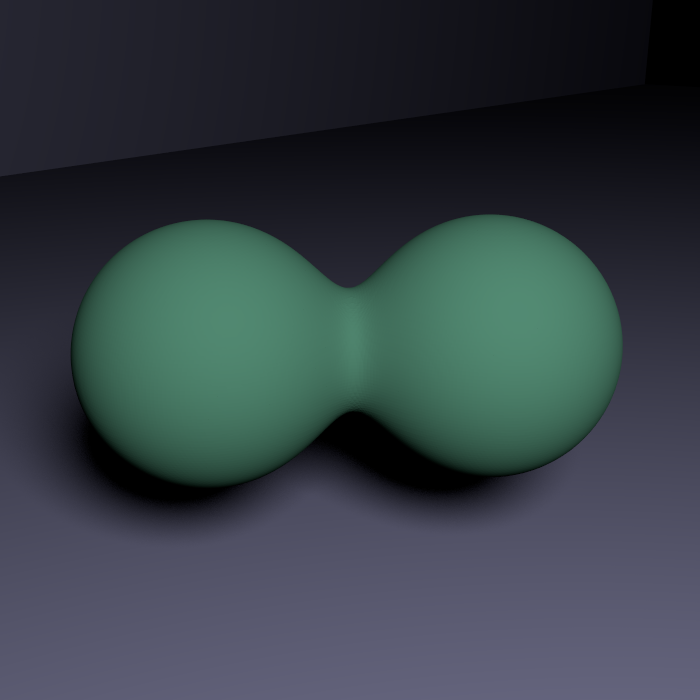
\includegraphics[width=1.5in]{images/metaball-good1.png}
  \caption{Mesh generated from metaball using the \textit{marching cubes} algorithm.}
  \label{img:marching-cubes}
\end{figure}

\subsection{Marching cubes implementation}

As seen before, the \textit{marching cubes} algorithm consists of dividing the
space in imaginary cubes, and then generating triangles in them considering
which of their vertices are within the surface. This demands two extra
parameters:

\begin{itemize}
  \item \textbf{\texttt{space}}: a vector defining the space analyzed by the algorithm
  \item \textbf{\texttt{step}}: the size of the cubes used in the algorithm
\end{itemize}

If the space is not big enough, part of the metaball may be cut out. On the
other hand, if it is too big, there will be too much wasted memory. The smaller
the step, the more precise the approzimated mesh will be, but also the more
memory and time the algorithm will consume. The overall time consumption of
applying our \textit{marching cubes} implementation to a metaball is
$O(\|\frac{space}{step}\|_\infty^3 n)$, where $n$ is the number of metaballs.
The memory space consumption is $O(\|\frac{space}{step}\|_\infty^3)$.

For code simplicity, we chose not to optimize the vertices calculations. That
is, we actually generate \textit{all} possible mesh vertices, and them construct
the index list (which defines the mesh's triangles) using it, practically always
leaving unused vertices. If the volume grid is $1000 \times 1000 \times 1000$,
this means that more or less three billion mesh vertices will be created. If
each vertex uses three floating-point numbers, that is roughly 12GB of memory
space.

A final note about this part of the implemantation is that we actually did not
cover all of the original \textit{marching cubes}' cases. Regardless, we still
achieved very good results for basic metaballs, which means that the remaining
cases are rare. We also do not calculate the vertex normals, which makes the
shading more faceted.

\subsection{Intersection implementation}

For the intersection, there are two major diffences comparing to the original
algorithm proposed by Blinn. The first is that PBRT does not requires
\texttt{Shape} implementations to find an intersection along a ray, but only
along a part of it. Thus, we needed to restrict the numerical methods iteration
to an interval of the ray's parameter.

The second difference is that, instead of using the hybrid method combining
Newton iterarion with \textit{regula falsi} iteration, we only used the second.
Blinn's reasoning for joining them is that Newton may diverge, while
\textit{regula falsi} slowly but surely converges. We tested with simple scenes
and found out that \textit{regula falsi}'s slowness was not enough to jeopardize
the render time considerably, thus being accetable for our project.

And that is all our implementation of this method does: find the intersection.
Since we could not find a global and generic parametrization for metaballs, we
could not provide PBRT with the proper differential geometry information. Since
the rendered images correctly show the metaballs' silhouette, it was enough to
show that Blinn's method implemention for calculating the intersection was
successful.

\section{Conclusion}

Lorem ipsum dolor sit amet, consectetur adipisicing elit, sed do
eiusmod tempor incididunt ut labore et dolore magna aliqua. Ut enim ad
minim veniam, quis nostrud exercitation ullamco laboris nisi ut
aliquip ex ea commodo consequat. Duis aute irure dolor in
reprehenderit in voluptate velit esse cillum dolore eu fugiat nulla
pariatur. Excepteur sint occaecat cupidatat non proident, sunt in
culpa qui officia deserunt mollit anim id est laborum.

\subsection{Results}

\begin{figure}[ht]
  \centering
  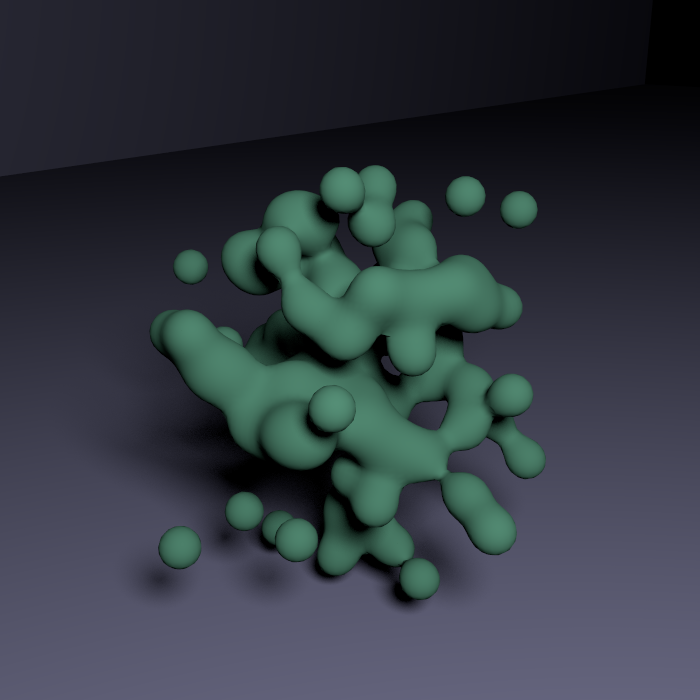
\includegraphics[width=1.5in]{images/blob.png}
  \caption{A complex set of metaballs rendered with our implementation}
  \label{img:blob}
\end{figure}

\subsection{Future works}

\section*{Acknowledgements}

%TODO

\bibliographystyle{acmsiggraph}
\bibliography{template}
\end{document}
